\documentclass[10pt]{article}
% \usepackage{geometry}
% \geometry{margin=0.2in}
\usepackage[utf8]{inputenc}

\nonstopmode
% \usepackage{minted}[cache=false]
\usepackage{graphicx} % Required for including pictures
\usepackage[figurename=Figure]{caption}
% \usepackage{float}    % For tables and other floats
\usepackage{amsmath}  % For math
\usepackage{amssymb}  % For more math
\usepackage{fullpage} % Set margins and place page numbers at bottom center
% \usepackage{paralist} % paragraph spacing
% \usepackage{subfig}   % For subfigures
%\usepackage{physics}  % for simplified dv, and 
% \usepackage{enumitem} % useful for itemization
% \usepackage{siunitx}  % standardization of si units
\usepackage{hyperref}
% \usepackage{mmacells}
% \usepackage{listings}
% \usepackage{svg}
% \usepackage{xcolor, soul}
\usepackage{bm}
\usepackage{braket}
% \usepackage{cancel}
% \usepackage{setspace}
% \usepackage{listings}
% \usepackage{listings}
% \usepackage[autoload=true]{jlcode}
% \usepackage{pygmentize}

% \definecolor{cambridgeblue}{rgb}{0.64, 0.76, 0.68}

% \sethlcolor{cambridgeblue}

\usepackage[margin=1.8cm]{geometry}
\newcommand{\C}{\mathbb C}
\newcommand{\D}{\bm D}
\newcommand{\R}{\mathbb R}
\newcommand{\Q}{\mathbb Q}
\newcommand{\Z}{\mathbb Z}
\newcommand{\N}{\mathbb N}
\newcommand{\PP}{\mathbb P}
\newcommand{\A}{\mathbb A}
\newcommand{\F}{\mathbb F}
\newcommand{\1}{\mathbf 1}
\newcommand{\ip}[1]{\left< #1 \right>}
\newcommand{\abs}[1]{\left| #1 \right|}
\newcommand{\norm}[1]{\left\| #1 \right\|}

\def\Tr{{\rm Tr}}
\def\tr{{\rm tr}}
\def\Var{{\rm Var}}
\def\calA{{\mathcal A}}
\def\calB{{\mathcal B}}
\def\calD{{\mathcal D}}
\def\calE{{\mathcal E}}
\def\calG{{\mathcal G}}
\def\from{{:}}
\def\lspan{{\rm span}}
\def\lrank{{\rm rank}}
\def\bd{{\rm bd}}
\def\acc{{\rm acc}}
\def\cl{{\rm cl}}
\def\sint{{\rm int}}
\def\ext{{\rm ext}}
\def\lnullity{{\rm nullity}}
% \DeclareSIUnit\clight{\text{\ensuremath{c}}}
% \DeclareSIUnit\fm{\femto\m}
% \DeclareSIUnit\hplanck{\text{\ensuremath{h}}}


% \lstdefinelanguage{julia}%
%   {morekeywords={abstract,break,case,catch,const,continue,do,else,elseif,%
%       end,export,false,for,function,immutable,import,importall,if,in,%
%       macro,module,otherwise,quote,return,switch,true,try,type,typealias,%
%       using,while},%
%    sensitive=true,%
% %    alsoother={$},%
%    morecomment=[l]\#,%
%    morecomment=[n]{\#=}{=\#},%
%    morestring=[s]{"}{"},%
%    morestring=[m]{'}{'},%
% }[keywords,comments,strings]%

% \lstset{%
%     language         = Julia,
%     basicstyle       = \ttfamily,
%     keywordstyle     = \bfseries\color{blue},
%     stringstyle      = \color{magenta},
%     commentstyle     = \color{ForestGreen},
%     showstringspaces = false,
% }

% $
\begin{document}
\begin{center}
	\hrule
	\vspace{.4cm}
	{\textbf { \large CAS PY 452 --- Quantum Physics II}}
\end{center}
Emmy Blumenthal \hspace{\fill} \hspace{\fill}  \textbf{} Discussion Notes\  \\
\textbf{Date:}\  Nov 9, 2022   \hspace{\fill} \textbf{Email:}\ emmyb320@bu.edu 
\vspace{.4cm}
\hrule

\section*{WKB wave-function and energies for the `quantum bouncing ball'}


\paragraph{Problem:}

Consider the `quantum bouncing ball.' That is, consider the single-particle system governed by the Hamiltonian, $\hat H = \frac{\hat p^2}{2m} + V(x)$, where the potential is,
\begin{align}
	V(x) = \begin{cases}
		m g x & x> 0\\
		\infty  & x \leq 0,
	\end{cases}
\end{align}
where $g>0$.
Find the WKB-approximation for the energies and wave-function.
Make a plot of the wave-function and compare to the analytical solution.

\paragraph{Solution:}

First, we find the WKB-approximated energy.
The semi-classical momentum when $x> 0$ is $p(x) = \sqrt{2m(E - mgx)}$.
There is a turning point at $x_1=0$ because $V(0) \to \infty$.
The other turning points occurs when,
\begin{align}
	p(x_2) = 0 \implies 
	x_2 = E/mg.
\end{align}
The Bohr-Sommerfeld quantization condition is,
\begin{gather}
	\int_0^{x_2} p(x) dx
	=
	\left(
		n - \frac{1}{4}
	\right)\pi \hbar
	\implies
	\sqrt{2m}
	\int_0^{E/mg}
	\sqrt{E - m g x}
	dx
	=
	-
	\frac{1}{gm}
	\sqrt{2m}
	\int_{E}^{0}
	\sqrt{u}
	du
	=
	\frac{2\sqrt{2}}{3g\sqrt{m}} E^{3/2}
	=
	\left(
		n - \frac{1}{4}
	\right) \pi \hbar\nonumber
	\\
	E_n = 
	\left(
		\frac{3\pi}{8\sqrt{2}}  \hbar g
		(4n-1)
	\right)^{2/3}
	% \implies 
	% E_4 = 
	% \left(
	% 	\frac{45\pi}{8\sqrt{2}} \hbar g
	% % \right)^{3/2}.
\end{gather}
To find the wave-function, we follow Griffiths section 9.2.
In the classically-allowed region (region I) ($E_n > V(x)$), the wave-function is,
\begin{align}
	\psi_\mathrm{I}(x) =
	\frac{A}{[2m(E_n - V(x))]^{1/4}}
	\sin(\int_x^{x_2} \sqrt{2m (E_n - V(x'))} dx' + \pi/4).
\end{align}
We are free to add the factor of $\pi/4$ as a constant of integration; similarly, we chose the limit of integration $x_2$ arbitrarily.
We choose a sine function with this phase-factor here because it will match the asymptotic expansions of the Airy functions.
% We chose a sine function here because we need $\psi_\mathrm{I}(0) = 0$ to satisfy boundary conditions.
In the classically-disallowed region (region III) ($V(x) > E_n$),
\begin{align}
	\psi_\mathrm{III}(x)
	=
	\frac{B}{[2m(V(x) - E_n)]^{1/4}}
	\exp(-\int_{x_2}^x \sqrt{2m(V(x') - E_n)} dx').
\end{align}
We need to deal with the `patching' region (region II) next.
We linearize the potential near the turning point: $V(x) \approx V(x_2) + (x-x_2) V'(x_2)
=
E_n + (x-x_2) V'(x_2)
$.
In this particular case, the approximation is exact because the potential is linear.
Near the turning point, we want to solve the TISE:
\begin{align}
	-\frac{\hbar^2}{2m}
	\frac{d^2\psi}{dx^2}
	+
	(E_n + (x-x_2)V'(x_2))
	\psi
	=
	E_n \psi
	\implies 
	\frac{\hbar^2}{2m V'(x_2)}
	\frac{d^2\psi}{dx^2}
	=
	% V'(x_2)
	(x-x_2)
	\psi.
\end{align}
By changing variables $\xi = (x-x_2)\alpha$, where $\alpha =[ 2mV'(x_2)/\hbar^2]^{1/3}$, this becomes,
\begin{align}
	\frac{d^2 \psi}{d\xi^2} = \xi \psi(\xi),
\end{align}
which has solutions $\psi = C\mathrm{Ai}(\xi) + D \mathrm{Bi}(\xi)$.

% By changing variables $\xi = (x-x_2)/\alpha$, where $\alpha = \sqrt{\hbar^2/(2m V'(x_2))}$,
% this becomes,
% \begin{align}
% 	\frac{d^2\psi}{d\xi^2}
% 	=
% 	\xi \psi(\xi),
% \end{align}
% which is Airy's equation which has solutions $\psi = C \mathrm{Ai}(\xi) + D \mathrm{Bi}(\xi)$.
The large positive $\xi$ (i.e., $x \gg x_2$) asymptotic expansion is,
\begin{align}
	\mathrm{Ai}(\xi)
	% =
	\sim
	\frac{e^{-\frac{2 \xi ^{3/2}}{3}}}{2 (\pi^2 \xi)^{1/4}},
	\qquad
	\mathrm{Bi}(\xi)
	% =
	\sim
	\frac{e^{\frac{2 \xi ^{3/2}}{3}}}{(\pi^2\xi)^{1/4}}.
\end{align}
To match to $\psi_{\mathrm{III}}(x)$, we must have $D = 0$ and,
\begin{align}
	\frac{C}{2(\pi^2 \xi)^{1/4}}
	=
	\frac{B}{(2m(V(x)- E_n))^{1/4}}.
\end{align}
The large negative $\xi$ asymptotic expansion is,
\begin{align}
	\mathrm{Ai}(\xi)
	\sim 
	\frac{1}{\sqrt{\pi}(-\xi)^{1/4}}
	\sin(\frac{2}{3}(-\xi)^{3/2} + \pi/4).
\end{align}
This means that,
\begin{align}
	\frac{C}{\sqrt{\pi}(-\xi)^{1/4}}
	=
	\frac{A}{(2m(E_n - V(x)))^{1/4}},
\end{align}
which gives us the relation between $A,B,C$.
Specifically, it gives us $A/C$ and $B/C$ so that there is only one common constant: $C$, which is determined by normalization.
Using all this, we can deduce the wave-function, but we have to choose the size of the `patching region.'
Note that the Bohr-Sommerfeld quantization condition for one `vertical wall' was derived by requiring $\psi_I(0) = 0$, so we have already implicitly taken care of boundary conditions.
The rest of the plotting and computation is continued in the attached {\em Mathematica} notebook.
See figure 1 for the results.
\begin{figure}[h!]
	\centering
	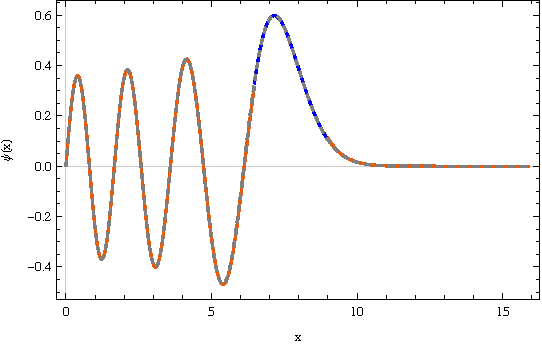
\includegraphics[width=0.8\linewidth]{plot.pdf}
	\caption{
		WKB compared to exact solution.
		Here, we show the exact solution using the gray-dotted line.
		The orange line represents the wave-function in region I and III.
		The blue line represents the patching region in region II.
		We see that are able to almost exactly replicate the exact solution.
	}
\end{figure}


\section*{The general (and numerical) approach to finding WKB energies}

If we want to find WKB estimations for the energies, we need to solve the Bohr-Sommerfeld quantization condition for the energies.
The process goes like this:

\paragraph{Write the semi-classical momentum $p(x,E) = \sqrt{2m[E - V(x)]}$.}
Here, we explicitly include write the energy $E$ as part of the momentum to remind us that we do not yet know the energy.

\paragraph{Find the turning points.}
The turning points occur when $E = V(x)$ or equivalently $p(x,E) = 0$.
This equation implicitly defines turning points $x_1(E)$ and $x_2(E)$ (where $x_1(E) < x_2(E)$) in terms of the so-far-unknown energy.
If there are vertical walls within the range of the relevant $E$, one or both of these turning points might be trivial (i.e., at the vertical wall).
% Note that there is a possibility that after a certain energy level, you might have to change from the case without vertical walls to the case with vertical walls.

\paragraph{Identify and solve the Bohr-Sommerfeld quantization condition.}
To obtain the $n$th energy (starting at $n=1$), we solve the equation:
\begin{align}
	\int_{x_1(E_n)}^{x_2(E_n)}
	p(x',E_n) dx'
	=
	\pi \hbar (n - \phi),
\end{align}
where $\phi = 0$ for two vertical walls at energy $E$, $\phi = \frac{1}{4}$ for one vertical wall at energy $E$, and $\phi = \frac{1}{2}$ for no vertical walls.
% I recommend trying to avoid using multiple quantization conditions in one problem; this might be accomplished by choosing your potential to be sufficiently `deep.'

% This equation can be solved numerically for $E$ if the integral and turning points are computed numerically.
% In {\em Mathematica}, you might do this with the functions `Range' to generate a list of energies, `NSolve' to find the turning points for each energy, `Interpolate' to turn the turning points vs. energies into a continuous function, `NIntegrate' to perform the integral on the LHS, and `FindRoot' to solve for the quantization condition; look at their documentations for more.


% This whole `vertical walls at energy $E$' can be summarized with this picture:

% \begin{center}
% 	\includegraphics[width=0.45\linewidth]{different_BS_conds.pdf}
% \end{center}



\section*{Numerically finding energies of the TISE}

To find the exact eigenvalues for a quantum system that is discretized as $x_1,\dots,x_n$ with spacing $dx$, we first define the `discrete Laplacian:'
\begin{align}
	\Delta = 
	\frac{1}{dx^2}
	\left(
		\begin{array}[]{cccccccccc}
			-2 & 1 & 0 & 0 &\cdots & 0 & 0 & 0 & 0\\
			1 & -2 & 1 & 0&\cdots & 0 & 0 & 0 & 0\\
			0 & 1 & -2 & 1 &\cdots & 0 & 0 & 0 & 0\\
			0 & 0 & 1 & -2 & \cdots & 0 & 0 & 0 & 0 \\
			\vdots & \vdots & \vdots & \vdots & \ddots & \vdots & \vdots & \vdots & \vdots \\
			0 & 0 & 0 & 0 & \cdots & -2 & 1 & 0 & 0 \\
			0 & 0 & 0 & 0 & \cdots & 1 & -2 & 1 & 0 \\
			0 & 0 & 0 & 0 & \cdots & 0 & 1 & -2 & 1 \\
			0 & 0 & 0 & 0 & \cdots & 0 & 0 & 1 & -2 \\
		\end{array}
	\right).
\end{align}
Note: the use of this form of the discrete Laplacian enforce `Dirichlet boundary conditions,' meaning that it pins the numerically-found eigenstates to zero at $x_1$ and $x_n$; this could also be interpreted as inserting an infinite potential barrier at the points.
The potential operator is,
\begin{align}
	\hat V
	=
	\left(
		\begin{array}{ccccc}
			V(x_1) & 0 & \cdots & 0 & 0\\
			0 & V(x_2)  & \cdots & 0 & 0\\
			\vdots & \vdots  & \ddots & \vdots & \vdots\\
			0 & 0  & \cdots & V(x_{n-1}) & 0\\
			0 & 0  & \cdots & 0 & V(x_n)\\
		\end{array}
	\right).
\end{align}
The total Hamiltonian is then a $n \times n$ matrix:
\begin{align}
	\hat H = -\frac{\hbar^2}{2m} \Delta + \hat V.
\end{align}
The eigenvalues of this operator are the energy eigenvalues and the eigenvectors are the stationary states.


% This equation gives the relationship between $C$ and $B$.
% Similarly, the large negative expansion of $\mathrm{Ai}(\xi)$ (i.e., $x \ll x_2$) is,
% \begin{align}
% 	\mathrm{Ai}(\xi)
% 	\sim
% 	\frac{1}{\sqrt{\pi}(-\xi)^{1/4}}
% 	\sin(\frac{2}{3}(-\xi)^{3/2} + \frac{\pi}{4}).
% \end{align}
% Matching with $\psi_\mathrm{I}(x)$ gives,
% \begin{align}
% 	\frac{C}{\sqrt{\pi}(-\xi)^{1/4}}
% 	=
% 	\frac{A}{[2m(E_n - V(x))]^{1/4}},
% \end{align}
% which tells us the relationship between $A$ and $C$.
% To get forms for these expressions and make plots, we use the attached {\em Mathematica} notebook; a key issue here is finding the appropriate width of the `patching' region.

% Generally,
% $ \int p(x) dx = - \frac{2\sqrt{2}}{3 g \sqrt{m}} (E - m g x)^{3/2} + C$, where $C$ is a constant of integration.
% This means that the WKB wave-function in the classical region (region I), is,
% \begin{align}
% 	\psi_\mathrm{I}(x)
% 	=
% 	\frac{A}{(2m(E_4 - m g x))^{1/4}} 
% 	\sin(\frac{2\sqrt{2}}{3g \sqrt{m}\hbar} (E_4 - m g x)^{3/2}
% 	+
% 	\frac{\pi}{4}),
% \end{align}
% where we are allowed to add the phase factor $\pi/4$ as the constant of integration.
% and the wave-function in the classically-disallowed region (region III) is,
% \begin{align}
% 	\psi_{\mathrm{III}}(x)
% 	=
% 	\frac{B}{(2m(m g x-E_4 ))^{1/4}} 
% 	\exp(-\frac{2\sqrt{2}}{3g \sqrt{m}\hbar} (m g x-E_4 )^{3/2}).
% \end{align}
% However, we have to `patch' the region (II) around the turning point by linearizing the potential: $V(x) \approx V(x_2) + V'(x_2) (x-x_2) = E_4 + m g (x - E_4/mg)$.
% Therefore, in the patching region, we need to solve the TISE:
% \begin{gather}
% 	-\frac{\hbar^2}{2m}\frac{d^2 \psi_\mathrm{II}}{dx^2}
% 	+ \left[
% 		E_4
% 		 +V'(x_2)(x-x_2)\right]\psi_\mathrm{II}(x) = E_4 \psi_\mathrm{II}(x)
% 	\\
% 	\implies
% 	\frac{\hbar^2}{2mV'(x_2)}
% 	\frac{d^2\psi_\mathrm{II}}{dx^2}
% 	=
% 	(x-x_2)
% 	\psi_\mathrm{II}(x)
% \end{gather}
% By changing variables $\xi = (x-x_2)/\sqrt{\hbar^2/(2m V'(x_2))} = (x-x_2)/\alpha$, this becomes $\frac{d^2\psi_\mathrm{II}}{d\xi^2} = \xi \psi_\mathrm{II}(\xi)$, which is `Airy's equation' and has solutions $\psi_\mathrm{II} (\xi) = D \mathrm{Ai}(\xi) + E\mathrm{Bi}(\xi)$.
% In the classical region, we use the large positive $\xi$ approximations:
% \begin{align}
% 	\mathrm{Ai}(\xi) \sim
% 	\frac{e^{-{2 \xi ^{3/2}}/{3}}}{2 (\pi^2 \xi)^{1/4}}
% 	,
% 	\qquad
% 	\mathrm{Bi}(\xi)
% 	\sim
% 	\frac{e^{{2 \xi ^{3/2}}/{3}}}{(\pi^2 \xi)^{1/4}}.
% \end{align}
% We must have $\psi_{\mathrm{II}} = D \mathrm{Ai}(\xi)$ for normalization.
% Additionally,
% \begin{align}
% 	\frac{B}{(2m(m g x-E_4 ))^{1/4}} 
% 	=
% 	\frac{D}{2(\pi^2 (x-E_4/mg)/\alpha)^{1/4 }}
% 	\implies
% 	\frac{B}{D}
% 	=
% 	\left(
% 		\frac{m^2 g \alpha}{8 \pi^2}
% 	\right)^{1/4}.
% \end{align}
% Similarly,
% the large negative $\xi$ asymptotic behavior of the Airy function is,
% \begin{align}
% 	\mathrm{Ai}(\xi)
% 	\sim
% 	\frac{1}{\sqrt{\pi}(-\xi)^{1/4}}
% 	\sin\left(
% 		\frac{2}{3}(-\xi)^{3/2} + \frac{\pi}{4}
% 	\right),
% \end{align}
% so we must have,
% \begin{align}
% 	\frac{A}{(2m(E_4-m g x ))^{1/4}}
% 	=
% 	\frac{D}{\sqrt{\pi}(E_4/mg - x)^{1/4}/\alpha^{1/4}}
% 	\implies
% 	\frac{A}{D}
% 	=
% 	\left(
% 		\frac{2gm^2\alpha}{\pi^2}
% 	\right)^{1/4}.
% \end{align}
% Additionally,
% \begin{align}
% 	\frac{\sqrt{2}}{g\sqrt{m}\hbar}(m g x - E_4)^{3/2}
% 	=
% 	2\xi^{3/2}/3
% 	=
% \end{align}
% Substituting $x = \xi \sqrt{\hbar^2/(2m V'(x_2))} + E/mg$ into our form for $\psi_\mathrm{I}$:
% \begin{align}
% 	\psi_\mathrm{I}(x)
% 	=
% \end{align}

% \begin{align}
% 	\int p(x) dx
% 	=
% 	\frac{}{}
% % \end{align}
% $\int p(x) dx =\sqrt{2m} \int \sqrt{E - m g x} dx = 
% \frac{2\sqrt{2}}{3g m } E^{3/2}$.
% In the case of $n =4$, $\int p(x) dx = \frac{2\sqrt{2}}{3g m } E_4^{3/2} = \frac{15}{4} \pi \hbar$


% \paragraph{Solution v2:}

% In the classically-allowed region (region I) ($E_n > V(x)$), the wave-function is,
% \begin{align}
% 	\psi_\mathrm{I}(x)
% 	=
% 	\frac{1}{[2m(E_n - V(x))]^{1/4}}
% 	\left[
% 	A_s
% 	\sin(\int^x \sqrt{2m(E_n - V(x'))}dx')
% 	+
% 	A_c
% 	\cos(\int^x \sqrt{2m(E_n - V(x'))}dx')
% 	\right].
% \end{align}
% Similarly, in the classically-disallowed region (region III) ($V(x) > E_n$),
% \begin{align}
% 	\psi_\mathrm{III}(x)
% 	=
% 	\frac{1}{[2m(V(x)-E_n )]^{1/4}}
% 	\left[
% 		B_-
% 		\exp(-\int^x \sqrt{2m(E_n - V(x'))}dx')
% 		+
% 		B_+
% 		\exp(+\int^x \sqrt{2m( V(x')-E_n)}dx')
% 	\right].
% \end{align}
% In order for $\psi_\mathrm{III}(x) \to 0$ as $x \to \infty$, we must have $B_+ = 0$.
% Next, we have to look at the `patching' region (region II).
% Here, we approximate the potential by linearizing about the turning point: $V(x) \approx V(x_2) + (x-x_2) V'(x_2)$.
% Near the turning point, we want to solve the TISE:
% \begin{align}
% 	-\frac{\hbar^2}{2m}
% 	\frac{d^2\psi}{dx^2}
% 	+
% 	(E_n + (x-x_2)V'(x_2))
% 	\psi
% 	=
% 	E_n \psi
% 	\implies 
% 	\frac{\hbar^2}{2m V'(x_2)}
% 	\frac{d^2\psi}{dx^2}
% 	=
% 	% V'(x_2)
% 	(x-x_2)
% 	\psi.
% \end{align}
% By changing variables $\xi = (x-x_2)\alpha$, where $\alpha =[ 2mV'(x_2)/\hbar^2]^{1/3}$, this becomes,
% \begin{align}
% 	\frac{d^2 \psi}{d\xi^2} = \xi \psi(\xi),
% \end{align}
% which has solutions $\psi = C\mathrm{Ai}(\xi) + D \mathrm{Bi}(\xi)$.
% The large positive $\xi$ (i.e., $x \gg x_2$) asymptotic expansion is,
% \begin{align}
% 	\mathrm{Ai}(\xi)
% 	% =
% 	\sim
% 	\frac{e^{-\frac{2 \xi ^{3/2}}{3}}}{2 (\pi^2 \xi)^{1/4}},
% 	\qquad
% 	\mathrm{Bi}(\xi)
% 	% =
% 	\sim
% 	\frac{e^{\frac{2 \xi ^{3/2}}{3}}}{(\pi^2\xi)^{1/4}}.
% \end{align}
% To match with $\psi_{\mathrm{III}}(x)$, we must have,
% \begin{align}
	
% \end{align}


\end{document}






